\iffalse
\documentclass[a4paper,12pt,twocolumn]{article}
\usepackage{graphicx}
\usepackage[margin=0.5in]{geometry}
\usepackage[cmex10]{amsmath}
\usepackage{array}
\usepackage{gensymb}
\usepackage{booktabs}
\usepackage{tabularx}
\title{Line Assignment}

\author{Ginna Shreyani- FWC22006}
\date{September 2022}
\providecommand{\norm}[1]{\left\lVert#1\right\rVert}
\providecommand{\abs}[1]{\left\vert#1\right\vert}
\let\vec\mathbf
\newcommand{\myvec}[1]{\ensuremath{\begin{pmatrix}#1\end{pmatrix}}}	
\newcommand{\mydet}[1]{\ensuremath{\begin{vmatrix}#1\end{vmatrix}}}
\providecommand{\brak}[1]{\ensuremath{\left((#1\right)}}
\begin{document}
\maketitle
\section{Problem:}
\fi
Diagonal AC of a parallelogram ABCD bisects $\angle{A}$ in Fig \eqref{fig:9/8/1/6}. Show that 
\begin{enumerate}
	\item	it bisects $\angle{C}$ also
	\item $ABCD$ is a rhombus
\end{enumerate}
\begin{figure}[!h]
	\centering
	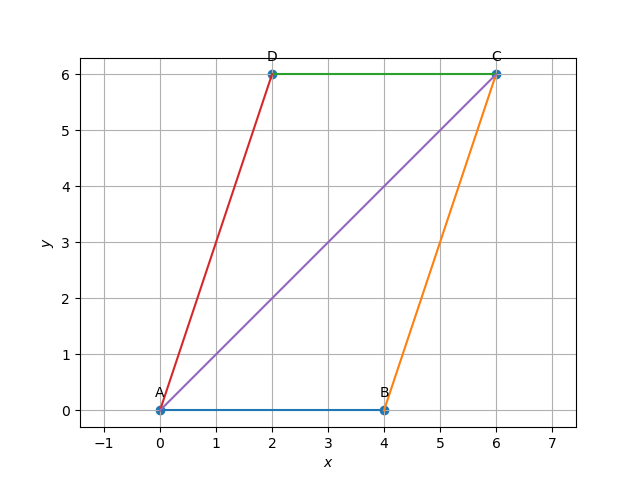
\includegraphics[width=\columnwidth]{chapters/9/8/1/6/figs/parallel.png}
	\caption{}
	\label{fig:9/8/1/6}
\end{figure}
\solution  
\iffalse
are given by 
\begin{proof}
Any point on the angle bisector is equidistant from the lines.  
\end{proof}
\fi	
%\item ({\em Reflection }) Assuming that straight lines work as a plane mirror for a point, find the image of the point $\vec{P}=\myvec{1\\2}$ in the line 
%%
\iffalse
\maketitle
\section{Construction:}
\begin{tabularx}
{0.5\textwidth}{
|>
{\raggedright\arraybackslash}X
|>
{\centering\arraybackslash}X
|>
{\raggedleft\arraybackslash}X
|}
\hline
 Variable & Point/Length & Description\\
\hline
 A  &  $\myvec{0\\0}$ & Vertex A\\
 \hline
 B & $\myvec{4\\0}$ & Vertex B\\
 \hline
 C & $\myvec{6\\6}$ & Vertex C\\
 \hline
 D & $\myvec{2\\6}$ & Vertex D\\
 \hline
\end{tabularx}
\maketitle
\section{Solution:}
\subsection{Theory:}
Given a diagonal of a parallelogram bisects an angle,we need to prove that the same diagonal bisects the opposite angle of the parallelogram by using vector algebra.\\
\subsection{Mathematical Calculation:}
Here the diagonal joining vertices A and C  can be represented as
\begin{equation}
\vec{C}-\vec{A} = \vec{B}-\vec{A}+\vec{C}-\vec{B}
\end{equation}
The other diagonal joining vertices B and D can be represented as
\begin{equation}
\vec{D-B} = \vec{B}-\vec{C}-\vec{B}-\vec{A}
\end{equation}
$\boldsymbol{(i)}$ Let the $\angle{CAB}$  be $\theta_1$ and the $\angle{DAC}$  be $\theta_2$ and the $\angle{DCA}$  be $\theta_3$ and $\angle{ACB}$ be $\theta_4$\\
Since the diagonal $\vec{C}-\vec{A}$ bisects $\angle{A}$, $\angle{CAB} = \angle{DAC}$,therefore we get $\theta_1=\theta_2$\\
\fi
\begin{enumerate}
	\item From 
    \eqref{eq:angle2d},
\begin{align}
	 \label{eq:9/8/1/6/bis}
	\angle{BAC}
	&= \angle{DAC}
	\\
\implies  \frac{(\vec{A}-\vec{B})^T(\vec{A}-\vec{C})}{\norm{\vec{A}-\vec{B}}\norm{\vec{A}-\vec{C}}}
	& = \frac{(\vec{A}-\vec{D})^T(\vec{A}-\vec{C})}{\norm{\vec{A}-\vec{D}}\norm{\vec{A}-\vec{C}}}
%
%&cos\theta_3 = \frac{\vec{-(B-A)}^T\vec{-(C-A)}}{\vec{||-(B-A)||}.\vec{||-(C-A)||}}\\
%&cos\theta_3 = \frac{\brak{vec{B}-\vec{A}}^T\brak{vec{C}-\vec{A}}}{\vec{||B-A||}.\vec{||C-A||}}\\
%&cos\theta_1 = cos\theta_3\\
%&\theta_1=\theta_3
\end{align}
Also, 
\begin{align}
\cos	\angle{ACD}
	 = \frac{(\vec{C}-\vec{D})^T(\vec{C}-\vec{A})}{\norm{\vec{C}-\vec{D}}\norm{\vec{C}-\vec{A}}}
	 \label{eq:9/8/1/6/cang}
%
\end{align}
From Appendix
	  \ref{eq:two-pgm}, 
  \begin{align}
	  \vec{B}-\vec{A} &= \vec{C} -\vec{D}
	  \\
	  \implies 
	  \frac{(\vec{C}-\vec{D})^T(\vec{C}-\vec{A})}{\norm{\vec{C}-\vec{D}}\norm{\vec{C}-\vec{A}}}
	  &= \frac{(\vec{B}-\vec{A})^T(\vec{C}-\vec{A})}{\norm{\vec{B}-\vec{A}}\norm{\vec{C}-\vec{A}}}
	 \label{eq:9/8/1/6/rh}
  \end{align}
  upon substituting in 
	 \eqref{eq:9/8/1/6/cang}. Thus, from 
	 \eqref{eq:9/8/1/6/cang}
	 and 
	 \eqref{eq:9/8/1/6/bis}, 
\begin{align}
	\angle{BAC}
	= \angle{DAC}
	=
	\angle{ACD}
  \end{align}
  Similarly, it can be shown that 
  \begin{align}
	\angle{ACD}
	=
	\angle{ACB}
  \end{align}
  \item 
  \iffalse
From 
	 \eqref{eq:9/8/1/6/rh}, 
  \begin{align}
	  \frac{(\vec{C}-\vec{D})^T(\vec{C}-\vec{A})}{\norm{\vec{C}-\vec{D}}\norm{\vec{C}-\vec{A}}}
	  &= \frac{(\vec{B}-\vec{A})^T(\vec{C}-\vec{A})}{\norm{\vec{B}-\vec{A}}\norm{\vec{C}-\vec{A}}}
  \end{align}
The equation of the bisector of $\angle BAD$ is given by Appendix  
	\ref{prob:ang-bisect} as
\begin{align}
	 \label{eq:9/8/1/6/ac}
	\frac{\vec{n}_1^{\top}\vec{x} - c_1}{\norm{\vec{n}_1}}
	= 
	\frac{\vec{n}_2^{\top}\vec{x} - c_2}{\norm{\vec{n}_2}}
\end{align}
where the equations of $AB, AD$ are respectively given by 
\begin{align}
	\vec{n}_1^{\top}\vec{x} &= c_1
	\\
	\vec{n}_2^{\top}\vec{x} &= c_2
\end{align}
From 
    \eqref{eq:dir_vec}
    and 
    \eqref{eq:normal_vec}, 
\begin{align}
	 \label{eq:9/8/1/6/orth}
	\vec{n}_1^{\top}\brak{\vec{A}-\vec{B}} &= 0
	\\
	\vec{n}_2^{\top}\brak{\vec{A}-\vec{D}}&= 0
\end{align}
%
From 
	 \eqref{eq:9/8/1/6/ac}, the normal vector of $AC$ is 
\begin{align}
	\frac{\vec{n}_1}{\norm{\vec{n}_1}}
	&- 
	\frac{\vec{n}_2}{\norm{\vec{n}_2}}
	\\
	\implies
	\brak{\frac{\vec{n}_1}{\norm{\vec{n}_1}}
	- 
	\frac{\vec{n}_2}{\norm{\vec{n}_2}}}^{\top}
\brak{\vec{B}-\vec{D}}
	&= 
	\brak{\frac{\vec{n}_1}{\norm{\vec{n}_1}}
	- 
	\frac{\vec{n}_2}{\norm{\vec{n}_2}}}^{\top}
	\sbrak{\brak{\vec{B}-\vec{A}}+
	\brak{\vec{A}-\vec{D}}}
\end{align}
which can be expressed as 
\begin{align}
	{\frac{\vec{n}_1^{\top}}{\norm{\vec{n}_1}}}\brak{\vec{A}-\vec{D}}
	- 
	\frac{\vec{n}_2^{\top}}{\norm{\vec{n}_2}}
	\brak{\vec{B}-\vec{A}}
\end{align}
upon substituting from 
	 \eqref{eq:9/8/1/6/orth}.
	 \fi

\end{enumerate}


\iffalse
Therefore,$\angle{CAB}=\angle{DAC}=\angle{DCA}$\\
Similarly, applying the same process to $\angle{DAC}$ and $\angle{ACB}$, we get $\theta_2=\theta_4$ and as result $\angle{DAC}=\angle{ACB}$.\\
Therefore, $\angle{DCA} = \angle{ACB}$\\
Since both the angles $\angle{DCA}$ and $\angle{ACB}$ are equal, we can conclude that the diagonal $\vec{C}-\vec{A}$ bisects the $\angle{C}$.\\ 
\end{document}
\fi
